\documentclass[class=article, crop=false]{standalone}
\usepackage[subpreambles=true]{standalone}
\usepackage{import}
\usepackage[T1]{fontenc}
\usepackage[utf8]{inputenc}
\usepackage[english, danish]{babel}
\usepackage{graphicx,wrapfig,lipsum}

\begin{document}
     I domænemodellen på figur~\ref{fig:domain_model} laves et overordnet indblik i spillet og hvad det skal indeholde. Dette bliver vist ved at inddele det i objekter der senere kan blive til klasser. De attributter og relationer der bliver vist giver overblik over informationen i programmet og vil senere vise sig i form af klassevariabler. \par
    Det afbilleder hvordan det ser ud i den virkelige verden, dog med små ændringer fra et egentligt Matadorspil - såsom maks antal af huse og “Kom ud af fængsel”-kort, der her kommer til at være essentielt uendeligt mange af. \par
    Normalt holder man sig helt fra tanker om selve programmet, men man kan tage ting generalisering op og se hvor det kan være praktisk at tage det i brug, som gjort her på felterne allerede her. Tanken er den samme som når der skal programmeres, hvor at der kan arves information af ‘super’-klasser.


    \begin{figure}[H]

                \hbox{\hspace{-1cm} 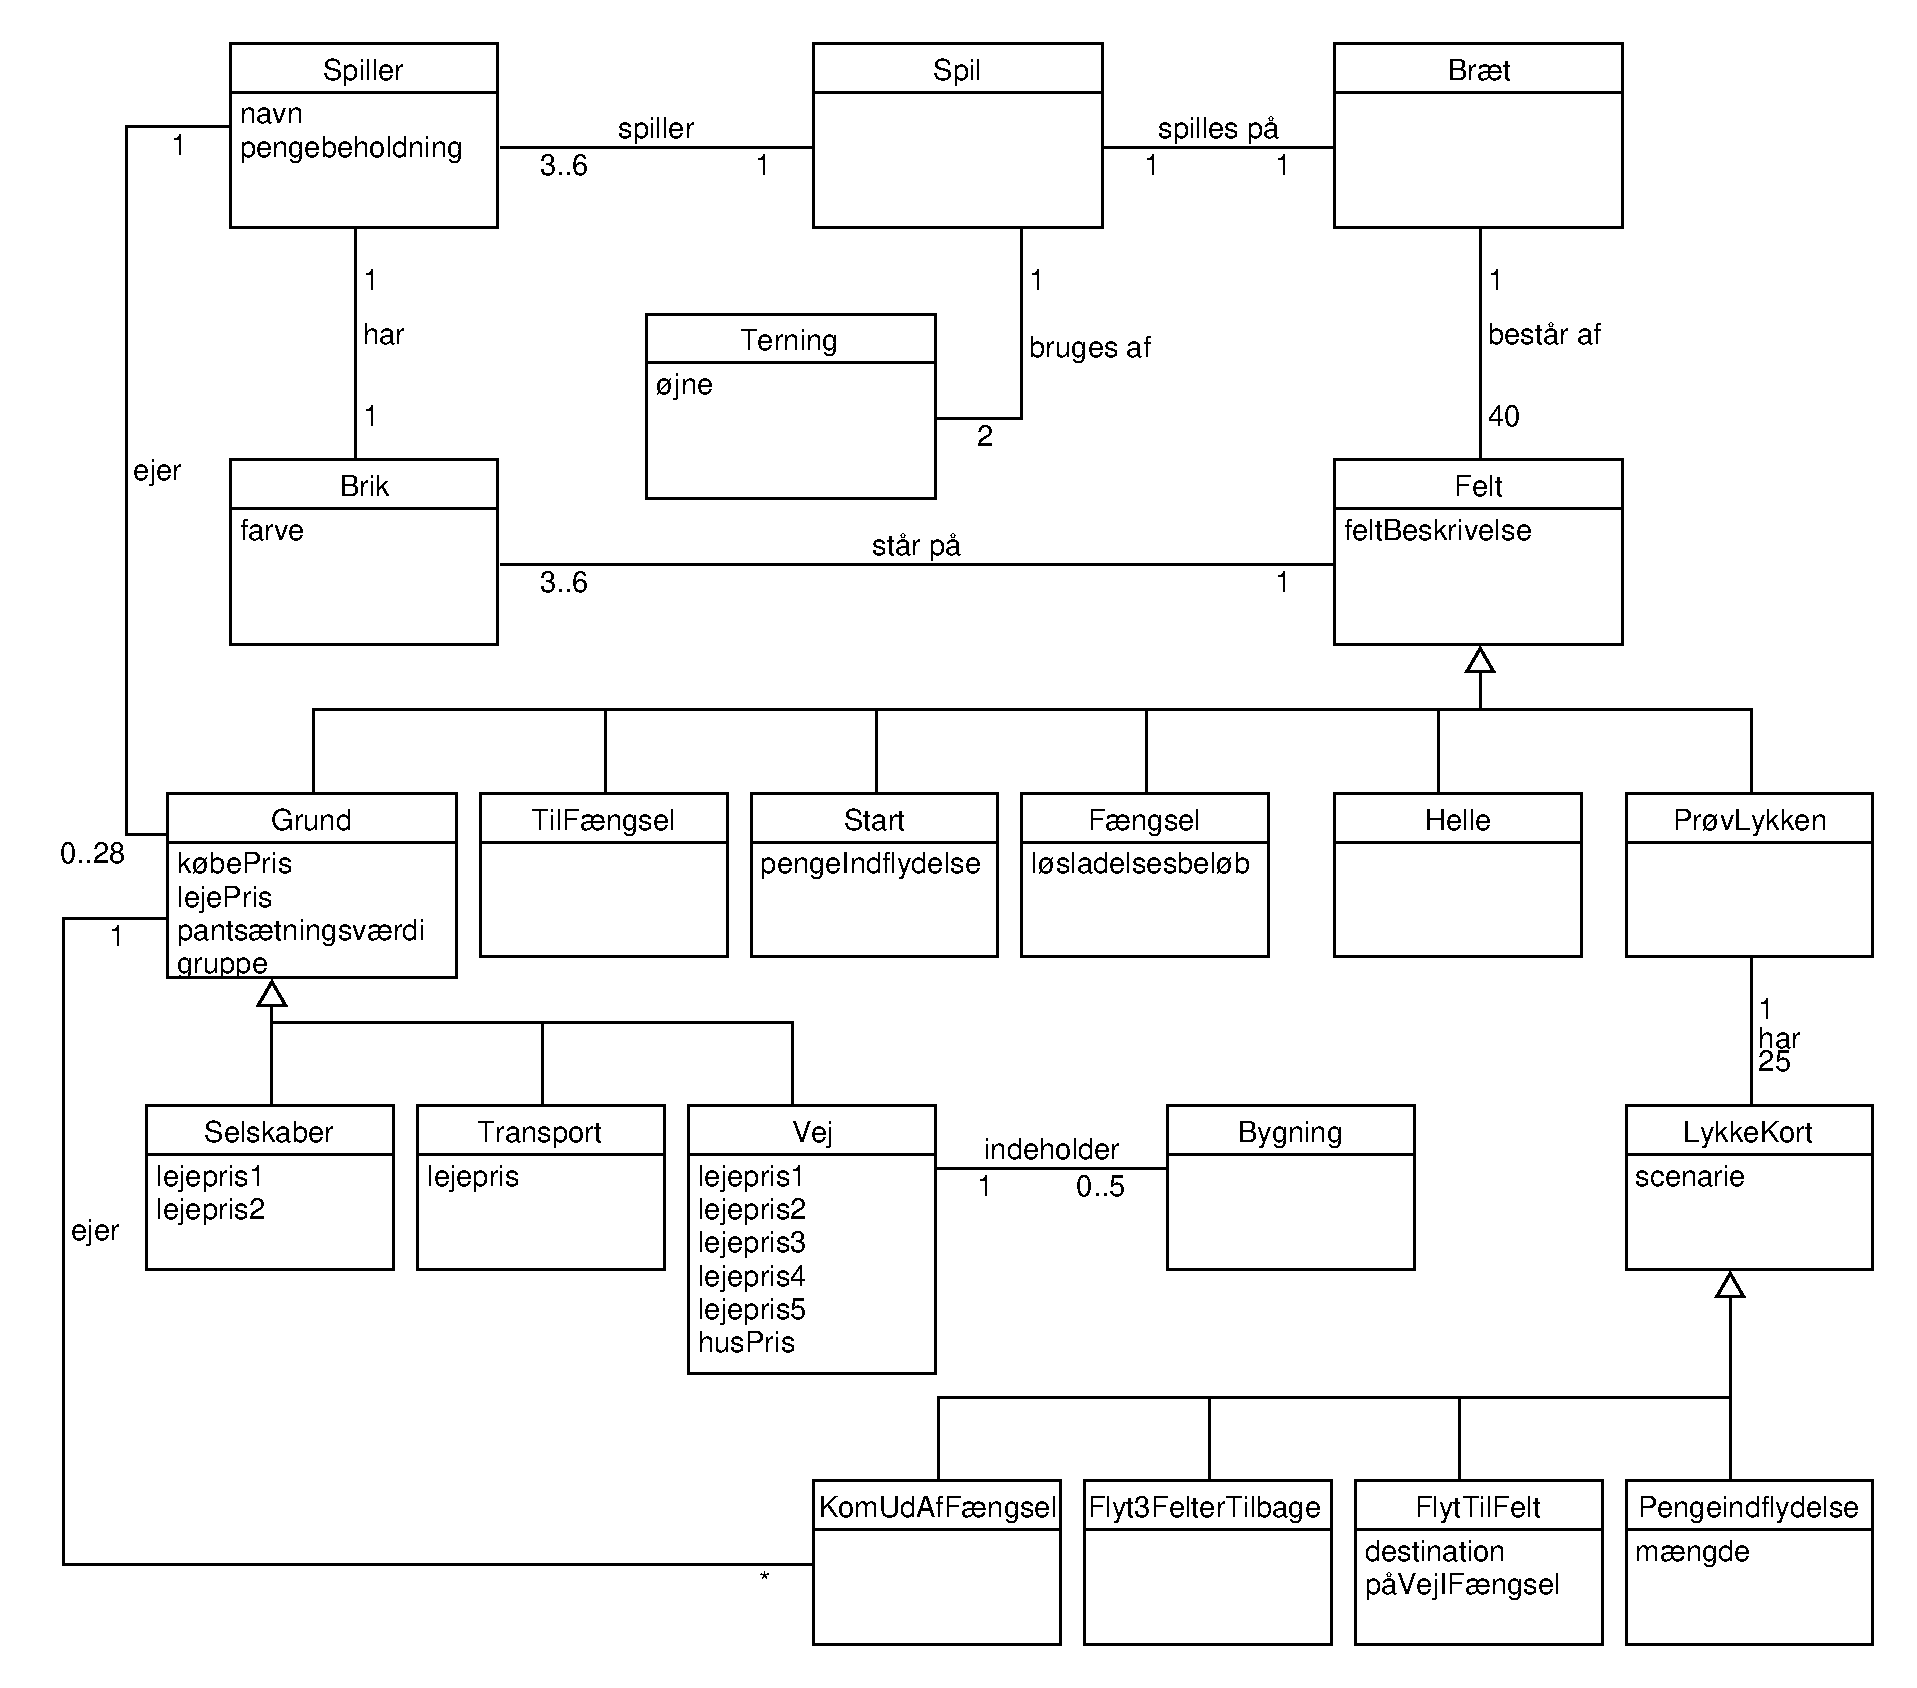
\includegraphics[scale=0.6]{diagrams/domain_model.pdf}}

                \caption{Domænemodellen over systemet}\label{fig:domain_model}
            \end{figure}

\end{document}